\message{ !name(paper.tex)}\documentclass[manuscript=cmatex]{achemso}
\usepackage[usenames,dvipsnames]{xcolor}
% \definecolor{linkcolor}{RGB}{0,0,240}
\usepackage{achemso}
\usepackage{makecell}
\usepackage{xr}
\usepackage{hyperref}
\usepackage{appendix}
\usepackage{upgreek}
\usepackage{chemmacros}
\usepackage{siunitx}
\usepackage{textcomp}
\usepackage{natmove}

\captionsetup{font={rm,small}}
\SectionNumbersOn
\usepackage[USenglish]{babel}
\addto\captionsenglish{\renewcommand\chaptername{Section}}
\usepackage{graphicx,array,tabularx,mathtools,siunitx,amsmath,multirow,longtable,float}
\usepackage[nameinlink,noabbrev,capitalize]{cleveref}
\setlength{\footskip}{0.25in}
\usepackage[labelformat=simple]{subfig}
\graphicspath{ {./imgs/} }
\usepackage{cleveref}
\usepackage[labelfont=bf]{caption}
\hypersetup{
  pdfstartview = {XYZ},
  allcolors = linkcolor,
  bookmarksopen,
  bookmarksnumbered,
  colorlinks=false,
  filecolor=black,
  citecolor = black,      
  urlcolor=black,
}

%%%%%%%%%%%%%%%%%%%%%%%%%%%%%%%%%%%%%%%% 
%%%%%%%%%%% 
% \numberwithin{reaction}{section}


\externaldocument[supp-]{si}



\title          {Evolution of Copper Surfaces under Plasma Oxidation: Molecular Dynamics Study with Neural Network Potentials}
\author         {Yantao Xia}
\affiliation    {Department of Chemical and Biomolecular Engineering, University of California, Los Angeles, CA 90095, USA}
\email          {xyttyxy@ucla.edu}
\author         {Philippe Sautet}
\affiliation    {Department of Chemical and Biomolecular Engineering, University of California, Los Angeles, CA 90095, USA}
\alsoaffiliation    {Department of Chemistry and Biochemistry, University of California, Los Angeles, CA 90095, USA}
\email          {sautet@ucla.edu}

%%%%%%%%%%%%%%%%%%%%%%%%%%%%%%%%%%%%%%%%%%%%%%%%%%% 
% table formatting commands
\renewcommand{\thesubfigure}{\relax} % no labels on subfigures
\begin{document}

\message{ !name(paper.tex) !offset(258) }
\begin{figure}[h]
  \centering
  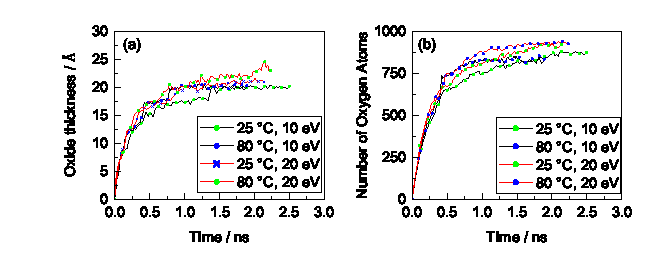
\includegraphics[width=\textwidth]{thicknumo_111.eps}
  \caption[Steinhardt's order parameter for slab]{Thickness and number of oxygen in the growing oxide on \ch{Cu} (111) surface. }
  \label{fig:thicknumo_111}
\end{figure}

\begin{figure}[h]
  \centering
  \includegraphics[width=\textwidth]{traj111}
  \caption[Oxidation trajectory on the Cu (111) surface]{Oxidation trajectory on the Cu (111) surface}
  \label{fig:traj111}
\end{figure}

\message{ !name(paper.tex) !offset(262) }

\end{document}

%%% Local Variables:
%%% mode: latex
%%% Tex-engine: xetex
%%% TeX-master: t
%%% End: